\documentclass[12pt]{article}
\usepackage{multirow}
\usepackage{graphicx}
\usepackage{times}
\usepackage[top=4cm,bottom=2cm,left=2cm,right=2cm]{geometry}
\parskip 6pt
\parindent 0pt
\usepackage{tweaklist}
\renewcommand{\itemhook}{\setlength{\topsep}{0pt} \setlength{\itemsep}{0pt}}
\renewcommand{\descripthook}{\setlength{\topsep}{0pt} \setlength{\itemsep}{0pt}}
\renewcommand{\enumhook}{\setlength{\topsep}{0pt} \setlength{\itemsep}{0pt}}

\title{Brontes Frame Grabber Design}
\author{Daniel Drake}
\date{\today}
\begin{document}
\maketitle

\section{Introduction}

The Frame Grabber (FG) will replace the costy and inconvenient IEEE1394-based image capture mechanism used in the Lava Chairside Oral Scanner (COS).

The FG will be custom designed as a PCI card, based on a Eureka PCI core. It will use direct memory access (DMA) to save frames into the computer memory.

Although this is an imaging device, the data transferred is arbitrary: the design makes no assumptions on what the data actually is.

This document details a suggested PCI-level interface to the FG.

\section{Overview}

\subsection{Block diagram}

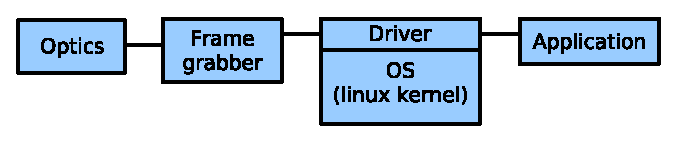
\includegraphics{block.eps}

\subsection{System overview}

The frame grabber is being built for the Lava Chairside Oral Scanner, a Linux-based embedded device running our own software with our own handheld optical peripheral device attached. The product allows teeth to be scanned in 3D for the purpose of constructing dental restorations (crowns, bridges, etc).

The optical peripheral is referred to as the "wand." The wand includes a microcontroller, an array of LEDs, some complicated optics, and some memory which stores some metadata (serial numbers, calibration data, etc). The wand is connected to the host computer over 2 interfaces:
\begin{enumerate}
\item The microcontroller is accessible over an RS232 interface, which we have connected to an internal USB-serial adapter. The microcontroller accepts commands to read/reflash the onboard memory, enable triggering (capture of image data), etc.
\item The optics side is accessible over the PCI bus as specified by this document. Previous versions of the product instead used IEEE1394.
\end{enumerate}

This document is primarily concerned with the PCI side. The microcontroller interface is of little relevance for PCI development, but do be aware that for the real wand, you must start image capture (triggering) by sending a command to the USB microcontroller.

The proprietary 3D imaging technology operates from an input of 3 images all captured at the same moment in time. You can view the system as having 3 cameras inside the wand. We currently capture images at resolution 1024x768 from each camera.

\subsection{Hardware}

The Eureka EC220 PCI core will be used by the FG. This hardware can act as both a master and target concurrently.

The bus master functionality will be used to write directly into system RAM, using DMA.

The bus target functionality will be used for the driver to request information (e.g. read registers) from the board. The EC220 forwards these requests to user logic.

The PCI configuration space is handled entirely by the EC220, independently of the user logic.

\subsection{Software}

This project includes the development of an OS-level driver for the hardware. This will be implemented as a Linux kernel driver.

The driver will handle:
\begin{itemize}
\item Hardware detection
\item Hardware initialization
\item Negotiation of DMA transfers
\item Communication of memory addresses to userspace
\end{itemize}

When triggered, the driver will reserve memory regions for frame transfer and communicate these to the hardware.

The driver will create a character device node, which will support mmap() to map the memory regions into userspace. An ioctl will be provided to determine which areas of the memory regions have data, and poll()/select() will be supported in order to notify userspace when the state of the memory regions changes.

At the driver level, this is a truly zero-copy mechanism: the driver itself does not touch the data, it just communicates the addresses of where the hardware put the image data to userspace.

As the driver will be linked against the Linux kernel, the driver itself must be open source, so we must be careful to exclude all sensitive IP from the driver. This should not be a problem given that the driver is simply transporting addresses of arbitrary lumps of data. The proprietary userspace code which uses the driver to locate the images (and then process them) is not bound to the Linux kernel licensing.

\subsection{Hardware/driver communication}

It is worth clarifying the only ways that the driver and the hardware can communicate.

\begin{description}
\item[DMA] The FG can write data into PC physical memory. This communication is invoked by the FG but the driver is not aware when this happens.
\item[Interrupt] The FG can generate an interrupt, which the driver is immediately made aware of. However, no data is passed with the interrupt.
\item[PCI read] The driver can submit read requests to the FG, which are passed to the user logic. The driver provides an address, then the FG immediately provides some data.
\item[PCI write] The driver can submit write requests to the FG, which are passed to user logic. The driver submits both an address and some data.
\end{description}

With these in mind, the driver-instantiated transfers are fairly easy to design: for reading information (e.g. the frame size), a PCI read to a predetermined address can be submitted. The FG will know that this address corresponds to frame size, and the user logic can return the correct result. For writing information (e.g. programming the addresses where the FG should DMA to), the driver can instantiate a PCI write to a predetermined address, with a physical memory address as data.

The FG-to-driver communication is a little less obvious. The FG can DMA to memory at will, but the driver is unaware of this event. The FG can generate the interrupt signal at will, but cannot pass any data alongside with the signal. The solution here is to combine some of the above: when the FG wants to communicate something to the driver, it will set some bits in an \textit{interrupt status register} and then send an interrupt to the system. Upon reception of an interrupt, the driver will examine the interrupt status register and act accordingly.

With these communication challenges understood, the suggested hardware design should be more understandable.

\subsection{Interrupt emission}

PCI is a shared bus, hence interrupt lines may be shared between different hardware devices. It is therefore important that if the FG generates an interrupt, the FG driver must be able to determine that the interrupt came from the FG (otherwise we risk accumulating unhandled interrupts, which crash the OS).

The hardware design should make a conscious effort to not generate more interrupts than strictly necessary.

The device should include a register to control whether interrupts are enabled or not, and this should default to disabled.

\subsection{PCI IDs}

Each PCI device has a series of identifiers generally used by drivers to identify the device and how it should communicate. The EC220 lets us specify our own IDs, and we should do so in a driver-friendly way.

\begin{description}
%FIXME
\item[Vendor ID] We will need to purchase our own vendor ID before production from the PCI SIG. During development, we can use the Eureka ID. (2 bytes)
\item[Product ID] Use of this field is left up to the owner of the vendor ID. We should get an initial value, and not change this unless the communications protocols between driver and FG change significantly. (2 bytes)
\item[Revision] We should use this as a version number, i.e. increment it when minor changes are made. However, if any of these changes affect the protocol significantly, we should change the product ID and reset the revision. (1 byte)
\item[Subvendor ID/Subproduct ID] I think the above fields provide enough versioning, we can reserve these for future use. (2 bytes each)
\end{description}

When Linux detects PCI hardware, it uses vendor/product/subvendor/subproduct codes in order to determine which driver should manage the device. The driver can then read the revision field later on.

Please ensure these guidelines are followed, as not doing so can cause some driver headaches. For example, some vendors reuse product IDs for vastly different devices which cannot even be driven by the same driver.

\section{Frame transfer}

\subsection{Triplets and frames}

I will use the term \textbf{triplet} to indicate a set of 3 memory regions which form a group of 3 images captured at one point in time.

I will use the term \textbf{frame} to refer to an individual image, a single memory region.

A triplet therefore consists of 3 frames. At a logical level, the FG presents data in triplet-sized units: it presents 3 perfectly synchronized frames at a time. This is in contrast to the previous IEEE1394-based system, where we effectively had 3 individual cameras and had to be very careful that the frames coming back from each camera were synchronized.

\subsection{Data transfer}

As mentioned above, DMA data transfers will be controlled by the driver. The FG will provide direct access to the EC220's DMA control registers through a certain portion of the PCI address space.

When the FG is ready to write a frame into system memory, the FG will set a bit in a status register and raise an interrupt. The driver will examine the status register, determine that a frame is ready to be copied into memory, and will proceed to program memory addresses and other details into the EC220 DMA control registers.

The FG logic will detect when the driver has enabled the start bit in the EC220 DMA status register, and will then start the transfer into RAM. When the transfer is complete, the FG will set a bit in a status register to indicate completion of the copy, and will then raise another interrupt.

The above description is only an overview, and is detailed programatically later in this document.

\section{Hardware}

\subsection{EC220 setup}

Table 4 (p7) of the EC220 documentation lists various signals that we should setup at hardware initialization time.

\subsubsection{BAR0\_SETUP}
We will use BAR0 to determine an address space for registers used for PCI read/write accesses from the driver.

\begin{description}
\item[Bit 34 (prefetchable)] Unset, for non-prefetchable
\item[Bit 33] Set, to enable the BAR
\item[Bit 32] Set, to appear as memory rather than ports
\item[Bits 31:16] Set to 0, 64K should be enough for anybody
\end{description}

\subsubsection{BAR1\_SETUP}
We will not use BAR1. Unset bit 33 to disable it.

\subsubsection{CLASS\_CODE}
Set to 0x040000 (Multimedia video controller, progif 0).

\subsubsection{DEVICE\_ID}
During development, set to 0x0001. Before production we will have to assign a final ID.

\subsubsection{INTERRUPT\_PIN}
FIXME Not sure what to put here

\subsubsection{REVISION\_ID}
Set to 0x0001 for initial version, increment when non-trivial changes are made.

\subsubsection{RUN\_66MHZ}
FIXME Not sure what to put here.

\subsubsection{SEL\_23}
FIXME not sure what to put here

\subsubsection{SUBSYSTEM\_ID and SUBVENDOR\_ID}
Set both to 0

\subsubsection{VENDOR\_ID}
During development, set to 0x1901 (Eureka). Before production, we will purchase our own vendor ID from the PCI SIG, which will be placed here.

\subsection{Registers}

BAR0 will contain the following 32-bit registers:

\begin{tabular}{|c|c|l|c|c|} \hline
\textbf{Offset} & \textbf{Mnemonic} & \textbf{Name} & \textbf{Default} & \textbf{Driver access} \\ \hline
0x00 & FRM\_SIZE & Frame size & 192 & RO \\ \hline
0x04 & HW\_CTRL & Hardware control & 0 & R/W \\ \hline
0x08 & DMA\_STS & DMA status & 0 & RO \\ \hline
0x0C & WAND\_STS & Wand status & 0 & RO \\ \hline
\end{tabular}

The registers at address 0x8000 upwards map to the EC220 DMA control registers
as follows:

\begin{tabular}{|c|c|} \hline
\textbf{BAR0 offset} & \textbf{EC220 register} \\ \hline
0x8000 & DMA Address Register \\ \hline
0x8004 & Transfer Size Register \\ \hline
0x8008 & DMA Status Register \\ \hline
\end{tabular}

\subsubsection{FRM\_SIZE}

\begin{description}
\item[Address] BAR0 + 0x0
\item[Driver access] RO
\item[Default value] 192
\item[Size] 32 bits
\end{description}

This register contains the size of a frame, expressed in terms of 4kb pages. The decimal value 192 should be hardwired here, 192*4096=1024*768=786432

This may need rethinking at some point in the future, because there are ongoing discussions about calibrating the device at a higher resolution. Right now, both the hardware and the driver make the assumption that the resolution is fixed and do not offer ways of requesting other resolutions.

\subsubsection{HW\_CTRL}

\begin{description}
\item[Address] BAR0 + 0x4
\item[Driver access] R/W
\item[Default value] 0
\item[Size] 32 bits
\end{description}

This flags register controls behaviour of the device.

\begin{tabular}{|c|c|c|}\hline
\textbf{Bit} & \textbf{Mnemonic} & \textbf{Description} \\ \hline
0 & FRM\_INT\_CTRL & Frame interrupt control \\ \hline
1 & CBL\_INT\_CTRL & Cable status interrupt control \\ \hline
2:31 & \multicolumn{2}{|c|}{Reserved} \\ \hline
\end{tabular}

\paragraph{FRM\_INT\_CTRL}

Set this bit to enable interrupt generation for frame transmission events. 

\paragraph{CBL\_INT\_CTRL}

Set this bit to enable interrupt generation for cable connection/disconnection events.

\subsubsection{DMA\_STS}

\begin{description}
\item[Address] BAR0 + 0x8
\item[Driver access] RO
\item[Default value] 0
\item[Size] 32 bits
\end{description}

Upon reception of an interrupt, the driver shall use the contents of this register to decide how to handle the interrupt.

With the eception of the NEXT\_TRF field, the contents of this register are reset to 0 when read by the driver.

\begin{tabular}{|c|c|c|} \hline
\textbf{Bit} & \textbf{Mnemonic} & \textbf{Description} \\ \hline
0:1 & NEXT\_TRF & One-based ID of next frame to be transferred. 0 = no frame pending \\ \hline
2 & DMA\_COMP & Completion of DMA transfer. \\ \hline
3 & CBL\_STS\_CHG & Cable status change. \\ \hline
4:7 & \multicolumn{2}{|c|}{Reserved} \\ \hline
% FIXME: TRP dropped might overflow
8:15 & TRP\_DROPPED & Triplets dropped counter. \\ \hline
16:31 & \multicolumn{2}{|c|}{Reserved} \\ \hline
\end{tabular}

\paragraph{NEXT\_TRF}

When nonzero, this field indicates that there is a frame ready to be transferred from the FG into system RAM. The value of the field indicates the one-based index into the triplet of the frame in question (the driver can use this value to determine when one triplet finishes and the next one starts). The driver shall proceed to program the DMA register in order to start the transfer.

When zero, this field indicates that there is currently no frame ready to be transferred into system RAM.

\paragraph{DMA\_COMP}

When the FG has completed a DMA transfer, it shall set this bit and raise an interrupt.

The driver shall not use this as an indication that the FG is ready to start the next DMA transfer. It only signifies completion of the previously programmed DMA operation.

\paragraph{CBL\_STS\_CHG}

Assuming that cable status interrupts are enabled in HW\_CTRL, the FG shall set this bit and generate an interrupt when the cable status changes (i.e. wand is connected or disconnected).

The driver can read the current cable status from the WAND\_STS register.

\paragraph{TRP\_DROPPED}

If the FG has to discard a triplet, it shall increment this counter by one.

This would happen when the device has not been able to completely transfer a triplet into system RAM before the next triplet arrives.

\subsubsection{WAND\_STS}

\begin{description}
\item[Address] BAR0 + 0xC
\item[Driver access] RO
\item[Default value] 0
\item[Size] 32 bits
\end{description}

\begin{tabular}{|c|c|c|} \hline
\textbf{Bit} & \textbf{Mnemonic} & \textbf{Description} \\ \hline
0 & WAND\_PRESENT & Wand presence \\ \hline
\end{tabular}

\paragraph{WAND\_PRESENT}

This bit will read 1 if a wand is connected, and 0 otherwise.

\subsection{Suggested hardware operation}

\subsubsection{Interrupt generation}

It is not mentioned explicitly below, but no interrupts shall ever be raised unless the relevant bit in \texttt{HW\_CTRL} is set. This applies to all events that generate interrupts.

In the image transfer case, an interrupt is raised for readiness of a frame to be copied into system memory, and another interrupt is raised to mark a DMA completion. There are cases described when both of these may happen simultaneously. It is legal for the device to generate a single interrupt in this case.

\subsubsection{Register accesses}

As identified in section 2, certain fields of certain registers must be reset to 0 after the current value has been supplied to the host system.

\subsubsection{Image capture}

The FG interface to start and stop image capture is not visible over the PCI bus. Instead, the USB-accessible microcontroller will start and stop image acquisition.

The FG shall capture 3 images simultaneously (one from each camera), and all of
these frames become "ready" in the FG internal memory at the same point in time, but these individual frames are presented to the system individually.

The FG shall proceed to capture a triplet into local buffers on the PCI board. When complete, the FG can start transferring these into RAM on the host computer. It shall first inform the system of the availability of a frame from camera 1, by setting \texttt{DMA\_STS:NEXT\_TRF} to 1 and raising an interrupt.

Immediately after, it is expected that the driver will negotiate the DMA transfer and write the appropriate values into the EC220 DMA registers. When the start bit is raised, the FG shall start the data transfer.

When the DMA transfer is complete, the FG shall set \texttt{DMA\_STS:DMA\_COMP}. The frame from camera 2 can now be transferred, so the FG shall set \texttt{DMA\_STS:NEXT\_TRF} to 2. At this point an interrupt shall be raised.
%FIXME ok to raise 2 above

Identically to frame 1, the driver will start the DMA transfer, the FG shall set \texttt{DMA\_STS:DMA\_COMP} when completed and raise another interrupt.

The process shall then repeat for frame 3, except \texttt{DMA\_STS:NEXT\_TRF} shall be set to 3 at the appropriate time. After the transfer of the 3rd frame has completed, the frame triplet has been completed successfully, and it is assumed that the next triplet is not yet ready to be transferred. At the completion of the 3rd frame copy into system RAM, \texttt{DMA\_STS:DMA\_COMP} shall be set, but \texttt{DMA\_STS:NEXT\_TRF} shall be left as 0.

The process repeats until frame transmission is disabled.

\subsubsection{Notes on concurrency}

The FG shall have two internal triplet buffers. The reasoning here is that we anticipate the DMA transfer will not be able to complete in the short amount of time we have after one capture cycle completes before the next one begins. Additionally, erroneous circumstances may occur where the driver is not able to program the DMA transfers quick enough, or it cannot reserve any more memory for DMA transfers, so we need a buffering system regardless.

Logically, the FG shall lock a triplet buffer as soon as it offers the first frame to the driver (by signalling an interrupt after setting \texttt{DMA\_STS:NEXT\_TRF}). It shall unlock the triplet after completion of transfer of the 3rd frame into system RAM (at which time it will set \texttt{DMA\_STS:DMA\_COMP} and raise an interrupt).

When a triplet buffer is locked, the FG shall not capture any images into it. The data there is locked into place until it is unlocked later.

As the FG will always transfer triplets sequentially, it is not possible under the design of this system for more than one triplet buffer to be locked at any one time. In other words, there will always be at least one triplet buffer unlocked where new data can be captured.

This may lead to the scenario where the contents of an unlocked frame triplet buffer need to be discarded because a new image is ready to be captured. This is by design, but will only happen under erroneous circumstances where the driver/OS is not able to keep up. The driver/OS will lose a number of triplets but it will be able to detect this and resume OK. See the scenarios below for further illustrations of this.

The following notation is used in the scenarios below:

\begin{itemize}
\item \textbf{B1} refers to internal buffer 1
\item \textbf{T1} refers to triplet 1
\item \textbf{T1F1} refers to triplet 1, frame 1
\end{itemize}

\paragraph{Scenario 1: DMA falls behind by 1 frame}
Something like the below is anticipated to happen all of the time. The system copes without dropping any frames.

\begin{enumerate}
\item Both B1 and B2 are unlocked and empty.
\item Image capture of T1 begins into B1.
\item Image capture of T1 completes.
\item B1 is locked. NEXT\_TRF is set to 1, interrupt raised.
\item Driver responds soon after, starts DMA transfer of T1F1.
\item Image capture of T2 begins. As B1 is locked, capture begins into B2.
\item DMA transfer of frame T1F1 completes. NEXT\_TRF is set to 2, DMA\_COMP is set, interrupt raised.
\item Driver responds soon after, starts DMA transfer of T1F2.
\item Image capture of T2 completes.
\item DMA transfer of frame T1F2 completes. NEXT\_TRF is set to 3, DMA\_COMP is set, interrupt raised.
\item Driver responds soon after, starts DMA transfer of T1F3.
\item DMA transfer of frame T1F3 completes. B1 (which held T1) is unlocked. B2 is locked. NEXT\_TRF is set to 1, DMA\_COMP is set, interrupt raised.
\item Driver responds soon after, starts DMA transfer of T2F1.
\item Image capture of T3 begins. As B2 is locked, capture begins into B1.
\item DMA transfer of frame T1F1 completes. NEXT\_TRF is set to 2, DMA\_COMP is set, interrupt raised.
\item Driver responds soon after, starts DMA transfer of T2F2.
\item ...
\end{enumerate}

The important points to note from the above is that image capture of T2 began before T1 had been completely copied into system RAM, but this did not hinder anything. When capture of T3 started, T2 had not been completely copied into system RAM, but the prior completion of T1 meant that there is a buffer available for capture.

\paragraph{Scenario 2: Unresponsive driver}

\begin{enumerate}
\item Both B1 (triplet buffer 1) and B2 (triplet buffer 2) are unlocked and empty.
\item Image capture of T1 begins into B1.
\item T1 image capture ends.
\item B1 is locked. NEXT\_TRF is set to 1, interrupt raised.
\item Time passes. Driver doesn't respond in any way.
\item Image capture of T2 begins. As B1 is locked, capture begins into B2.
\item Image capture of T2 into B2 completes. As the transfer from B1 is still ongoing (actually, it hasn't even started), no interrupt is raised.
\item Time passes. Driver still hasn't responded.
\item Image capture of T3 begins. As B1 is locked, capture begins into B2. As B2 already contained a triplet, this triplet is discarded and TRP\_DROPPED is incremented.
\item Image capture into B2 completes. As the transfer from B1 is still ongoing (actually, it hasn't even started), no interrupt is raised.
\item ...
\end{enumerate}

\paragraph{Scenario 3: Unresponsive driver recovery}

\begin{enumerate}
\item T1 is captured into B1. B1 is locked. Driver starts DMA transfers, the copy of the first frame has completed and the 2nd (T1F2) is in progress.
\item T2 capture begins into B2.
\item DMA transfer of T1F2 completes. NEXT\_TRF is set to 3, DMA\_COMP is set, interrupt raised.
\item Driver does not respond for some reason.
\item T2 capture (into B2) completes.
\item T3 capture begins. B1 is still locked, so capture happens into B2. There was already a triplet in B2, so TRP\_DROPPED is incremented.
\item Driver finally programs new DMA buffers. Transfer of T1F3 begins.
\item Transfer of T1F3 completes. DMA\_COMP is set, interrupt raised. At this point, there is not currently any triplet ready to be transferred.
\item Driver receives interrupt, reads registers and observes that TRP\_DROPPED is non-zero (i.e. a frame has been lost).
\item Capture of T3 completes. NEXT\_TRF is set to 1, interrupt raised.
\item Driver starts DMA transfer of T3F1.
\item ...
\end{enumerate}

Interesting points above: When the DMA transfer of T2 completed, the FG was not ready to transfer the next triplet as the capture had not completed. Two interrupts were required where under other circumstances one might have done -- the first to indicate copy completion of T2F3, and the 2nd a little while later to indicate the availability of T3F1.

\subsection{Suggested driver operation}

\subsubsection{Initialization}

The driver shall read the frame size from \texttt{FRM\_SIZE} and reserve a series of appropriately sized physically contiguous segments in memory.

\subsubsection{Enabling image transmission}

When ready to process images, the driver shall set the \texttt{FRM\_INT\_CTRL} bit in \texttt{HW\_CTRL}. Image acqusition will actually start when the software later sends a command to the microcontroller over the USB bus (out of the scope of the document).

\subsubsection{Interrupt handling}

Upon reception of an interrupt, the driver shall read the value of \textbf{DMA\_STS}. If this register reads 0, the interrupt handler should exit with a status code indicating that the driver did not handle the interrupt.

Otherwise, the driver must handle the interrupt.

If \textbf{DMA\_STS:NEXT\_TRF} is nonzero, the driver shall try it's best to program the DMA registers with the address of a free frame in system RAM and start the transfer. The driver shall note the value of this field, as it is used to keep track of which parts of the current triplet have been transferred.

It may be the case that the driver is not able to program further frame addresses into the device, because those memory regions are not available (e.g. userspace is still using them). In this case, the driver should not take any action on the hardware, but could possibly record a flag to be communicated to it's users later. The users can determine the number of discarded frames by reading \texttt{TRP\_DROPPED}.

If \textbf{DMA\_STS:DMA\_COMP} is nonzero, the driver shall observe that the previously-programmed DMA transfer was completed successfully. By tracking the value of \texttt{NEXT\_TRF} throughout, it shall realise that this particular completion may mark the completion of a triplet, in which case it is able to hand off that data to userspace.

\subsubsection{Ending transmission}

When the image capture session is to be terminated, the driver shall clear the \texttt{INT\_CTRL} bit in the \texttt{HW\_CTRL} register. The driver shall then read \texttt{TRP\_DROPPED} in order to reset its value.

It is assumed that the higher level software will have already stopped image acqusition by sending a command to the microcontroller over the USB bus.

\subsubsection{User functionality}

The driver shall provide the following functionality to it's users:

\begin{enumerate}
\item A mechanism to address the memory frames programmed into the device.
\item A mechanism to control which frames are programmed at any one time.
\item A mechanism to read \texttt{TRP\_DROPPED}.
\end{enumerate}

\section{Driver specification}

\subsection{Buffer theory}

To remain somewhat analogous to the current IEEE1394-based software code, we will use the term \textit{buffer} to refer to a triplet.

During component initialization, the application will request a number of buffers from the driver. The driver will then attempt to reserve the appropriate amount of segments in physical memory.

When referenced in other interfaces, buffers will be referenced by index, starting at 0.

The driver will provide \texttt{mmap} functionality to modify the application processes \textit{virtual address space}. It will provide a region, contiguous in virtual memory, which will contiguously address the buffers in numerical order (and contiguously address their segments within). In other words, it will allow the application to obtain a memory map in it's virtual address space which looks as follows:

\begin{tabular}{|c|c|c|}\hline
Buffer 1 Frame 1 & Buffer 1 Frame 2 & Buffer 1 Frame 3 \\ \hline
Buffer 2 Frame 1 & Buffer 2 Frame 2 & Buffer 2 Frame 3 \\ \hline
Buffer 3 Frame 1 & Buffer 3 Frame 2 & Buffer 3 Frame 3 \\ \hline
\end{tabular}

In the above table, each row is one buffer (i.e. one triplet), and each cell is one image frame. Each cell is positioned in virtual memory immediately after the end of the previous one.

Buffers have a notion of \textit{ownership} which may initially seem a little unintuitive.
\begin{itemize}
\item Immediately after being allocated by the driver, all buffers are owned by the application.
\item For buffers owned by the application, the application can ask the driver to \textit{queue} such buffers at will. Buffers which have been queued are owned by the driver.
\item The application should never touch memory in buffers that it does not own. Such behaviour is undefined.
\item The driver shall ask the FG to write data into buffers which it owns, in the order that they were queued from the driver.
\item When the driver observes that the FG has finished copying a frame triplet into system RAM, ownership of the corresponding buffer is automatically assigned to the application.
\end{itemize}

\subsection{Initializing}

The b3dfg module will define a \texttt{pci\_driver} with an ID table including the vendor and product IDs defined by the hardware.

The \texttt{module\_init} function will create a device class named \texttt{b3dfg}. \texttt{alloc\_chrdev\_region()} will be used to allocate a character device region with a dynamic major.

\subsection{Probing}

A private \texttt{b3dfg\_dev} structure will be allocated during probe, used to store the per-device information.

A devno will be allocated based on the earlier-allocated dynamic major, and a dynamic minor.

A character device will be initialized and then assigned the devno using \texttt{cdev\_init()} and \texttt{cdev\_add()}. A b3dfg class device will then be created with the same devno.

Finally, the PCI device will be enabled using \texttt{pci\_enable\_device()} and the per-device \texttt{b3dfg\_dev} is stored in the device private data using \texttt{pci\_set\_drvdata}.

\subsection{Character device file operations}

\subsubsection{open}

Other than storing a reference to the b3dfg\_dev structure in the file pointer, open() is almost a no-op here.

\subsubsection{ioctl}

\paragraph{GET\_BUFFER\_SIZE}

This ioctl shall return the size of a single buffer.

\paragraph{SET\_BUFFERS}

This ioctl shall be used to allocate a number of buffers in memory. Further invocations shall change the number of allocated buffers (by allocating more or freeing existing ones). This can only be called when transmission is disabled and will dequeue any buffers that have been queued.

\paragraph{QUEUE\_BUFFER}

This ioctl shall transfer control of a buffer from the application to the FG. Some time later, during image transmission, this buffer shall fill up with a frame triplet.

\paragraph{POLL\_BUFFER}

This non-blocking ioctl shall examine the status of a queued buffer and indicate whether image data has arrived or not.

\paragraph{WAIT\_BUFFER}

This blocking ioctl shall examine the status of a queued buffer. If it has been filled with image data, it shall return immediately indicating this. Otherwise, it shall wait until image data arrives and then return.

\paragraph{SET\_TRANSMISSION}

This ioctl shall enable or disable image transmission.

\paragraph{GET\_DROPPED}

This ioctl shall be used to query the number of buffers dropped by the hardware.

\subsubsection{mmap}

% FIXME: mmap and SET_BUFFERS incompatibilities?
mmap shall provide a nopage function which will provide a memory region in the processes virtual address space which corresponds to the allocated buffers represented contiguously.

\subsubsection{poll}

poll shall add a waitqueue entry which triggers as soon as an image is transferred into any buffer.

\subsubsection{close}

This is almost a no-op apart from cleaning up.

\end{document}

